\chapter{Floppy Disks And D81 Images}
\label{cha:freezer}

\phantomsection

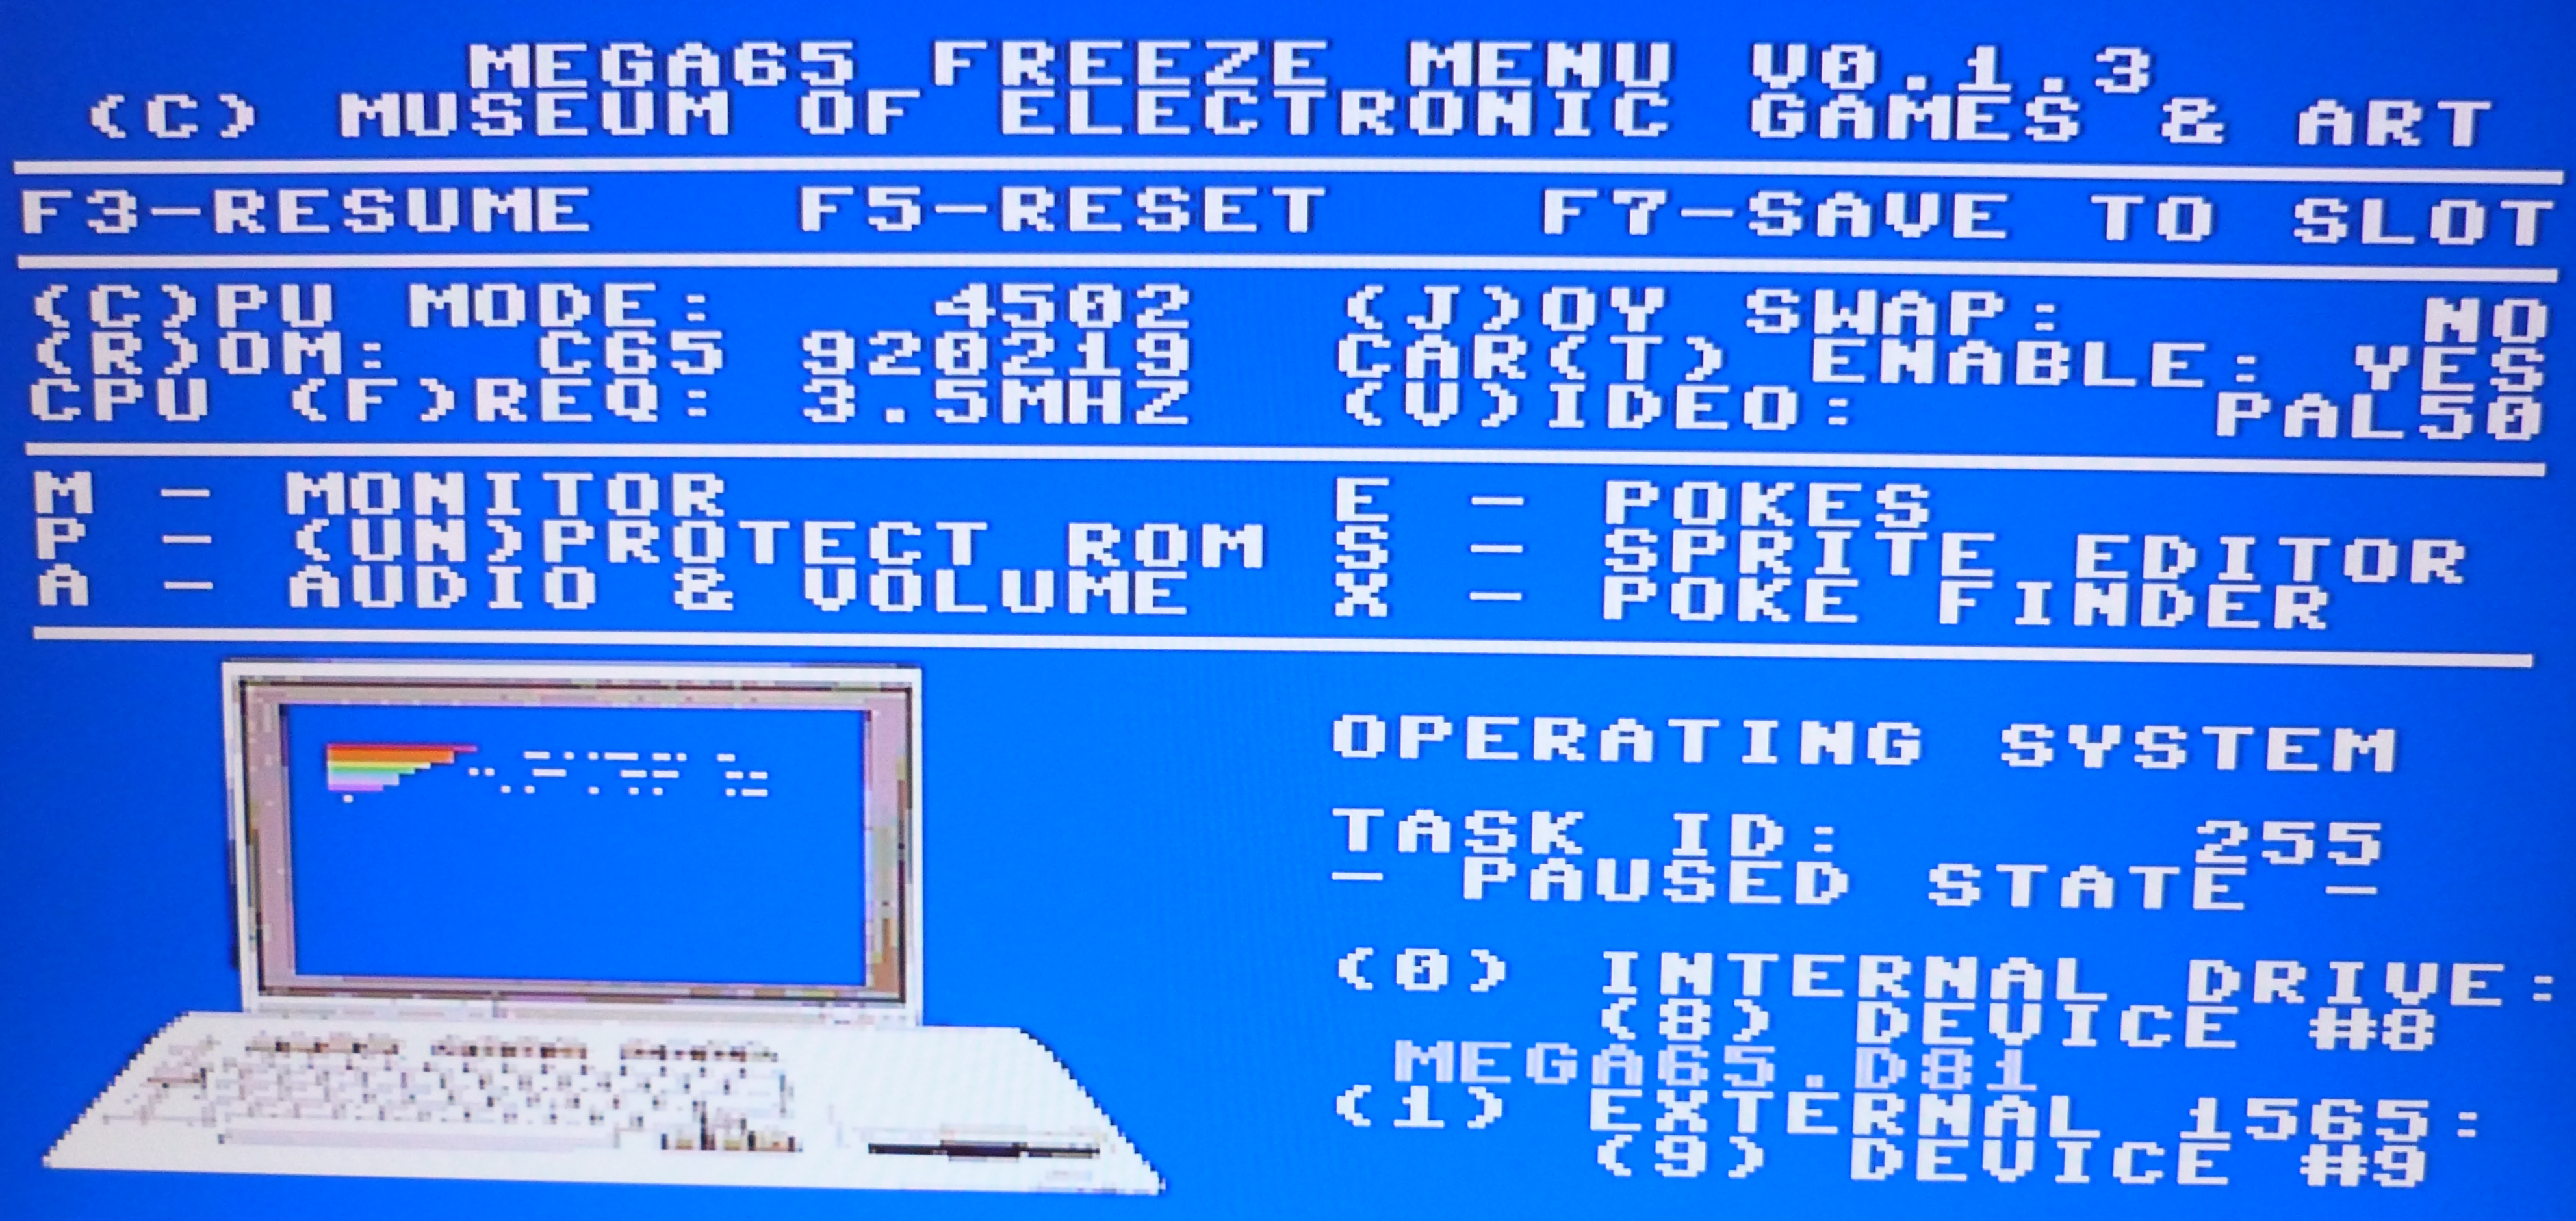
\includegraphics[width=\linewidth]{images/freezer.jpg}

\section{Terminology}

{\bf BASIC} and {\bf CBDOS} use following terminology:

{\bf UNIT} is a device number in the range 0-31.
The numbers from 0 to 11 are reserved for following device types:

{\ttfamily
\setlength{\tabcolsep}{1mm}
\begin{tabular}{|l|l|l|}
\hline
 unit \# & device  & comment \\
\hline
0        & KEYBOARD & input \\
1        & unused   & was TAPE on C64 \\
2        & unused   & was RS232 on C64 \\
3        & SCREEN   & input/output     \\
4-5      & IEC PRINTER  & output     \\
6-7      & IEC PLOTTER  & output     \\
8-9      & CBDOS drives & floppy drive or disk image \\
10-11    & IEC drives   & 1541, 1571, 1581, FD-2000 \\
\hline
\end{tabular}
}

{\bf DRIVE} is the drive number in a dual drive unit.
The drive number can be 0 or 1 only.
There are no dual drive units with IEC interface,
so the drive number for devices like 1541 or 1581 is always 0.

Dual disk drives like 4040, 8050, 8250 which use drive numbers
0 and 1 are equipped with the IEEE-488 interface and need
an IEEE-488 to IEC converter to be used on the MEGA65.

The internal floppy controller of the MEGA65 can control
two floppy drives (one internal and one external, both attached to the same
ribbon cable). The {\bf FREEZER} can be used to assign D81 images from the
SD-card to the drive numbers 0 and/or 1, instead of physical floppy drives.

BASIC commands, that address files or disks, use therefore
{\bf U} for UNIT and {\bf D} for drive.
The default settings are {\bf UNIT = 8} and {\bf DRIVE = 0}.

\section{The Freezer}

\section{Internal Floppy Disk Drive}

\section{Disk Images}

\section{Unit Assignment}


